\documentclass[12pt]{article}

\input preamble

\title{Principles of Parallel Architecture\\
Fine Grain Synchronization}
\author{Xitong Liu \\
xliu@ece.udel.edu}

\begin{document}

\maketitle

\section{Dataflow}
Write a dataflow program that receives a token that contains an 
array with N numbers and produces these outputs:
\begin{enumerate}
\end{enumerate}
\subsection{Average}
\begin{figure}[h!]
	\begin{center}
		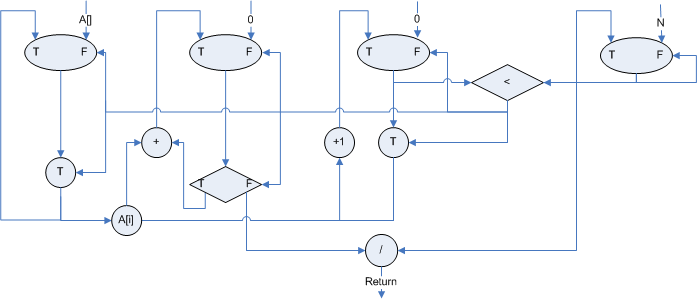
\includegraphics[width=1.0\textwidth, angle=0]{average.png}
		\caption{\label{fig:png}Dataflow Program of Array Average}
	\end{center}
\end{figure}
\subsection{Standard Deviation}

\end{document}

\begin{comment}
\begin{figure}[h!]
	\begin{center}
		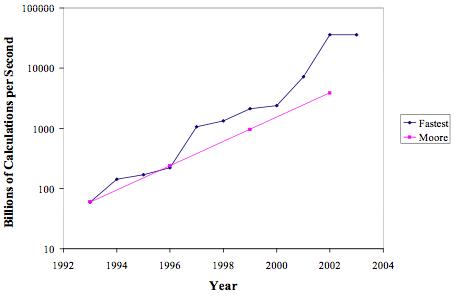
\includegraphics[width=0.7\textwidth, angle=0]{fatest.png}
		\caption{\label{fig:fatest}Fatest SuperComputer in the world}
	\end{center}
\end{figure}
\end{comment}